\documentclass[12pt]{article}
\usepackage[utf8]{inputenc}
\usepackage{cite}
\usepackage[utf8]{inputenc}
\usepackage{graphicx}
\usepackage{amsmath}
\pagenumbering{gobble}
\usepackage[margin=0.5in]{geometry}
\usepackage{multirow}
%\usepackage{geometry}
\usepackage{pdfpages}
\usepackage{xcolor}
\usepackage{todonotes}
\usepackage{amsmath,amsfonts,amssymb,amsthm,epsfig,epstopdf,titling,url,array}
\setcounter{secnumdepth}{4}
%\usepackage{enumerate}% http://ctan.org/pkg/enumerate
\title{Models of Decision Making}
\author{Joan Reyero}
%\date{\today}

\newtheorem*{theorem}{Theorem}


\newcommand\MyBox[1]{%
  \fbox{\parbox[c][1.7cm][c]{1.7cm}{\centering #1}}%
}
\newcommand\MyVBox[1]{%
  \parbox[c][1.7cm][c]{1cm}{\centering\bfseries #1}%
}  
\newcommand\MyHBox[2][\dimexpr1.7cm+2\fboxsep\relax]{%
  \parbox[c][1cm][c]{#1}{\centering\bfseries #2}%
}  
\newcommand\MyTBox[4]{%
  \MyVBox{#1}\MyBox{#2}\hspace*{-\fboxrule}%
  \MyBox{#3}\hspace*{-\fboxrule}%
  \MyBox{#4}\par\vspace{-\fboxrule}
}  



\bibliographystyle{apalike}
%\bibliography{bib}


\begin{document}

\maketitle

\section{Drift decision process}

This section will model a decision process between two hypotheses, $h^+$ and $h^-$, using a Wiener diffusion process. 

\subsection{Initial simulations}
\begin{figure}[h!]
	\centering
	\hspace*{-0.6in}
	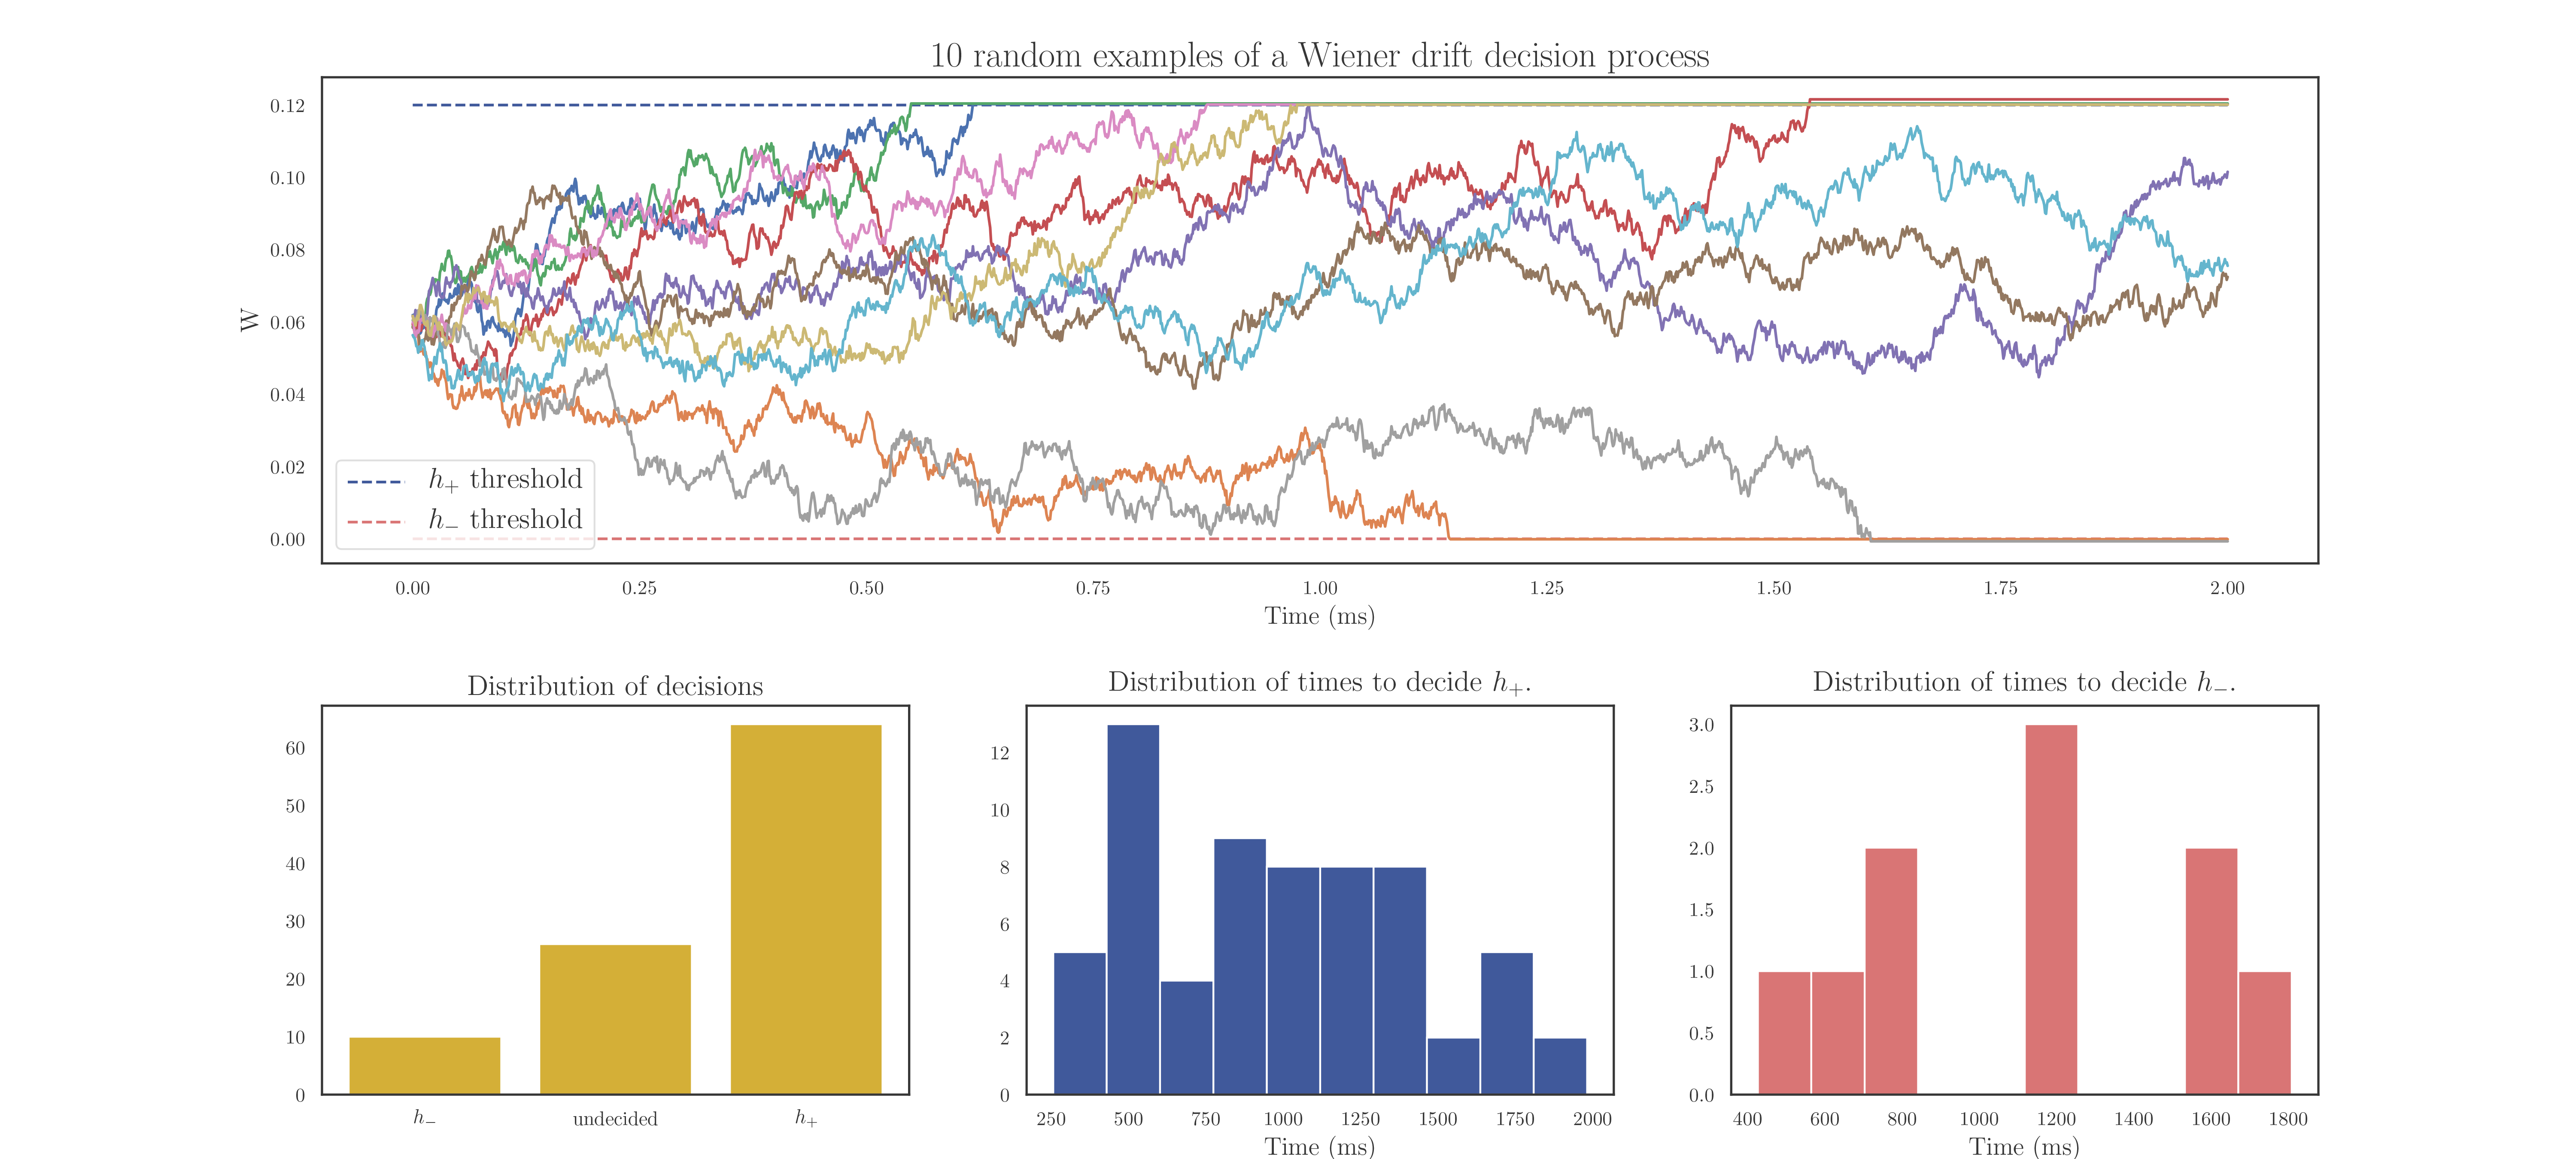
\includegraphics[width=1.2\linewidth]{figures/1-initial.png}
	\caption{Results of a drift-decision simulation ran 100 times with a drift-diffusion rate of 0.03 and a boundary separation of 0.12. Top: 10 randomly chosen decision paths. Bottom-left: Overall distribution of $h^+$, undecided and $h^-$. Bottom-centre: distribution of times to decide $h^+$. Bottom-right: distribution of times to decide $h^-$.}
	\label{fig:1-initial}
\end{figure}

Figure \ref{fig:1-initial} shows the 10 random example paths of a simulation ran 100 times, the overall distribution of the decisions, and the distribution of the times taken for each decision. Most processes have $h^+$ as the final decision, although some stay undecided or tend towards $h^-$, and a big variability due to noise is shown. The times to reach decision one are mainly distributed between 250 and 1500ms, while the times to reach decision 2 look more random, as they are caused only due to the random Gaussian noise.

The exact distribution is shown below:

\begin{itemize}
    \item $h^+$: 64 out of 100
    \item undecided: 26 out of 100
    \item $h^-$: 10 out of 100
\end{itemize}


From this results we can infer that the evidence that is being accumulated points towards $h^+$, although it is distorted by the noise – either to stay undecided or to not reach a decision – almost 40\% of the time.

\subsection{Parameter settings exploration}

To explore the effect of the mean drift rate, $v$, and the boundary separation, $a$, several simulations were conducted with different parameter settings:

The resulting distributions can be seen in the table below:

\begin{center}
 \begin{tabular}{|c || c | c | c | c |} 
 \hline
  & $(v=0.06, a=0.12)$ & $(v=0.06, a=0.06)$ & $(v=0.03, a=0.06)$ & $(v=0.0, a=0.06)$ \\ [0.5ex] 
 \hline\hline
 $h^+$ (\%)    & 91 & 90 & 80 & 56 \\ 
 \hline
 Undecided (\%)& 9  & 1  & 0  & 3  \\
 \hline
 $h^-$ (\%)    & 0  & 9  & 20 & 41 \\ [1ex]
 \hline
\end{tabular}
\end{center}

\begin{description}
    \item[Doubling $v$ but leaving $a$ the same $(v=0.06, a=0.12)$] results in 91\% of decisions towards $h^+$, as there is double the evidence. The reaction times were quicker than with the original parameters due the increased evidence (figure \ref{1-params} (A)). 
    \item[Doubling $v$ and halving $a$ $(v=0.06, a=0.06)$] As before, it has a high $h^+$ rate due to it having double the evidence. However, the random noise has a lot more effect due to the smaller boundary, so almost all the undecided states go to $h^-$. The reaction times were even quicker than before because we added the narrower bound (figure \ref{1-params} (B))
    \item[Leaving $v$ the same and halving $a$ $(v=0.03, a=0.06)$] results in having no undecided states, as the decision boundary is smaller. $h^-$ is double the original parameter values, due to the noise having a greater effect because of the smaller decision boundary. The reaction times were quicker than with the original parameters, concentrated around 500ms (figure \ref{1-params} (C)), but this time for both $h^+$ and $h^-$ due to the narrow bounds but having the original evidence.
    \item[Setting $v$ to 0 and halving $a$ $(v=0.0, a=0.06)$] There is no evidence and all of the decisions are made with the random noise, so it spreads evenly between $h^+$ and $h^-$. The decision times are equally distributed around 500ms for both hypothesis (figure \ref{1-params} (D)).
\end{description}

\begin{figure}[h!]
	\centering
	\hspace*{-0.6in}
	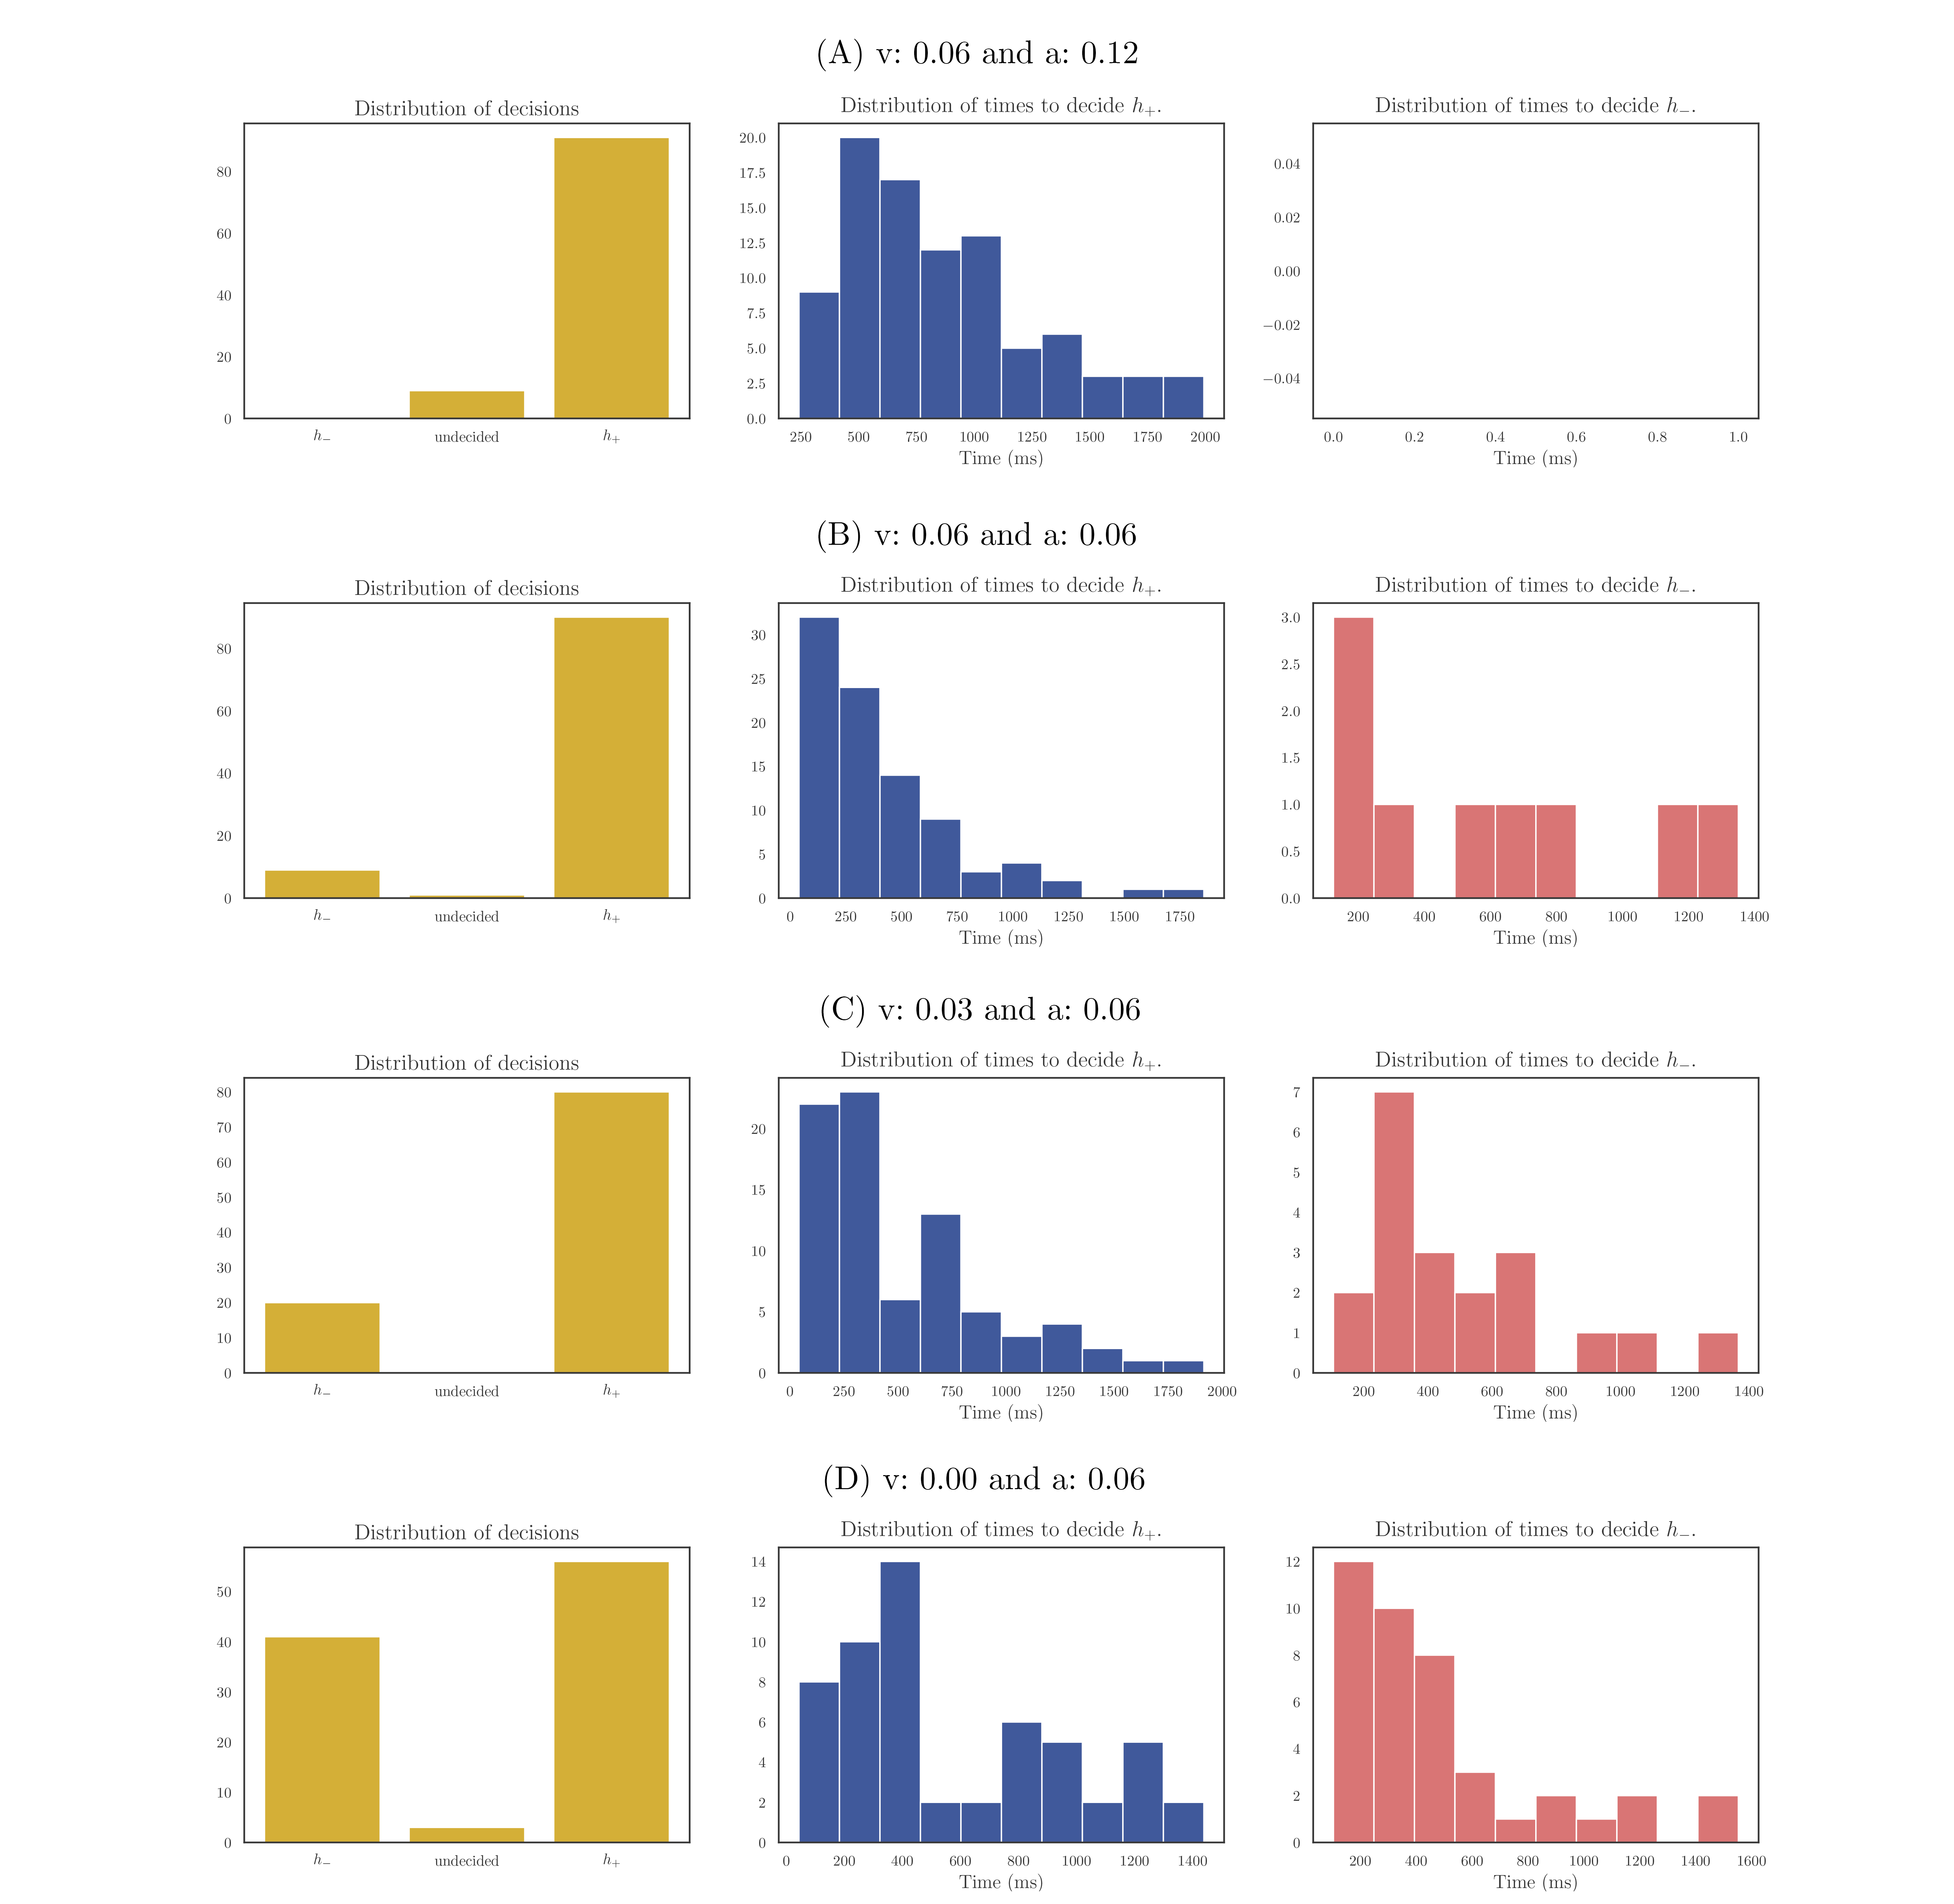
\includegraphics[width=1.2\linewidth]{figures/1-params.png}
	\caption{Distributions of decisions and times to make the decisions for different parameter settings.}
	\label{1-params}
\end{figure}

\subsection{Adding bias}

In order to add a bias such that the prior of $h^+$ is double the prior of $h^-$, it is sufficient to mode $z=\frac{2a}{3}$. This way, the distance from $z$ to $a$ will be half the distance from $z$ to $0$, which will make the prior of $h^+$ double than the prior of $h^-$.

\begin{figure}[h!]
	\centering
	\hspace*{-0.6in}
	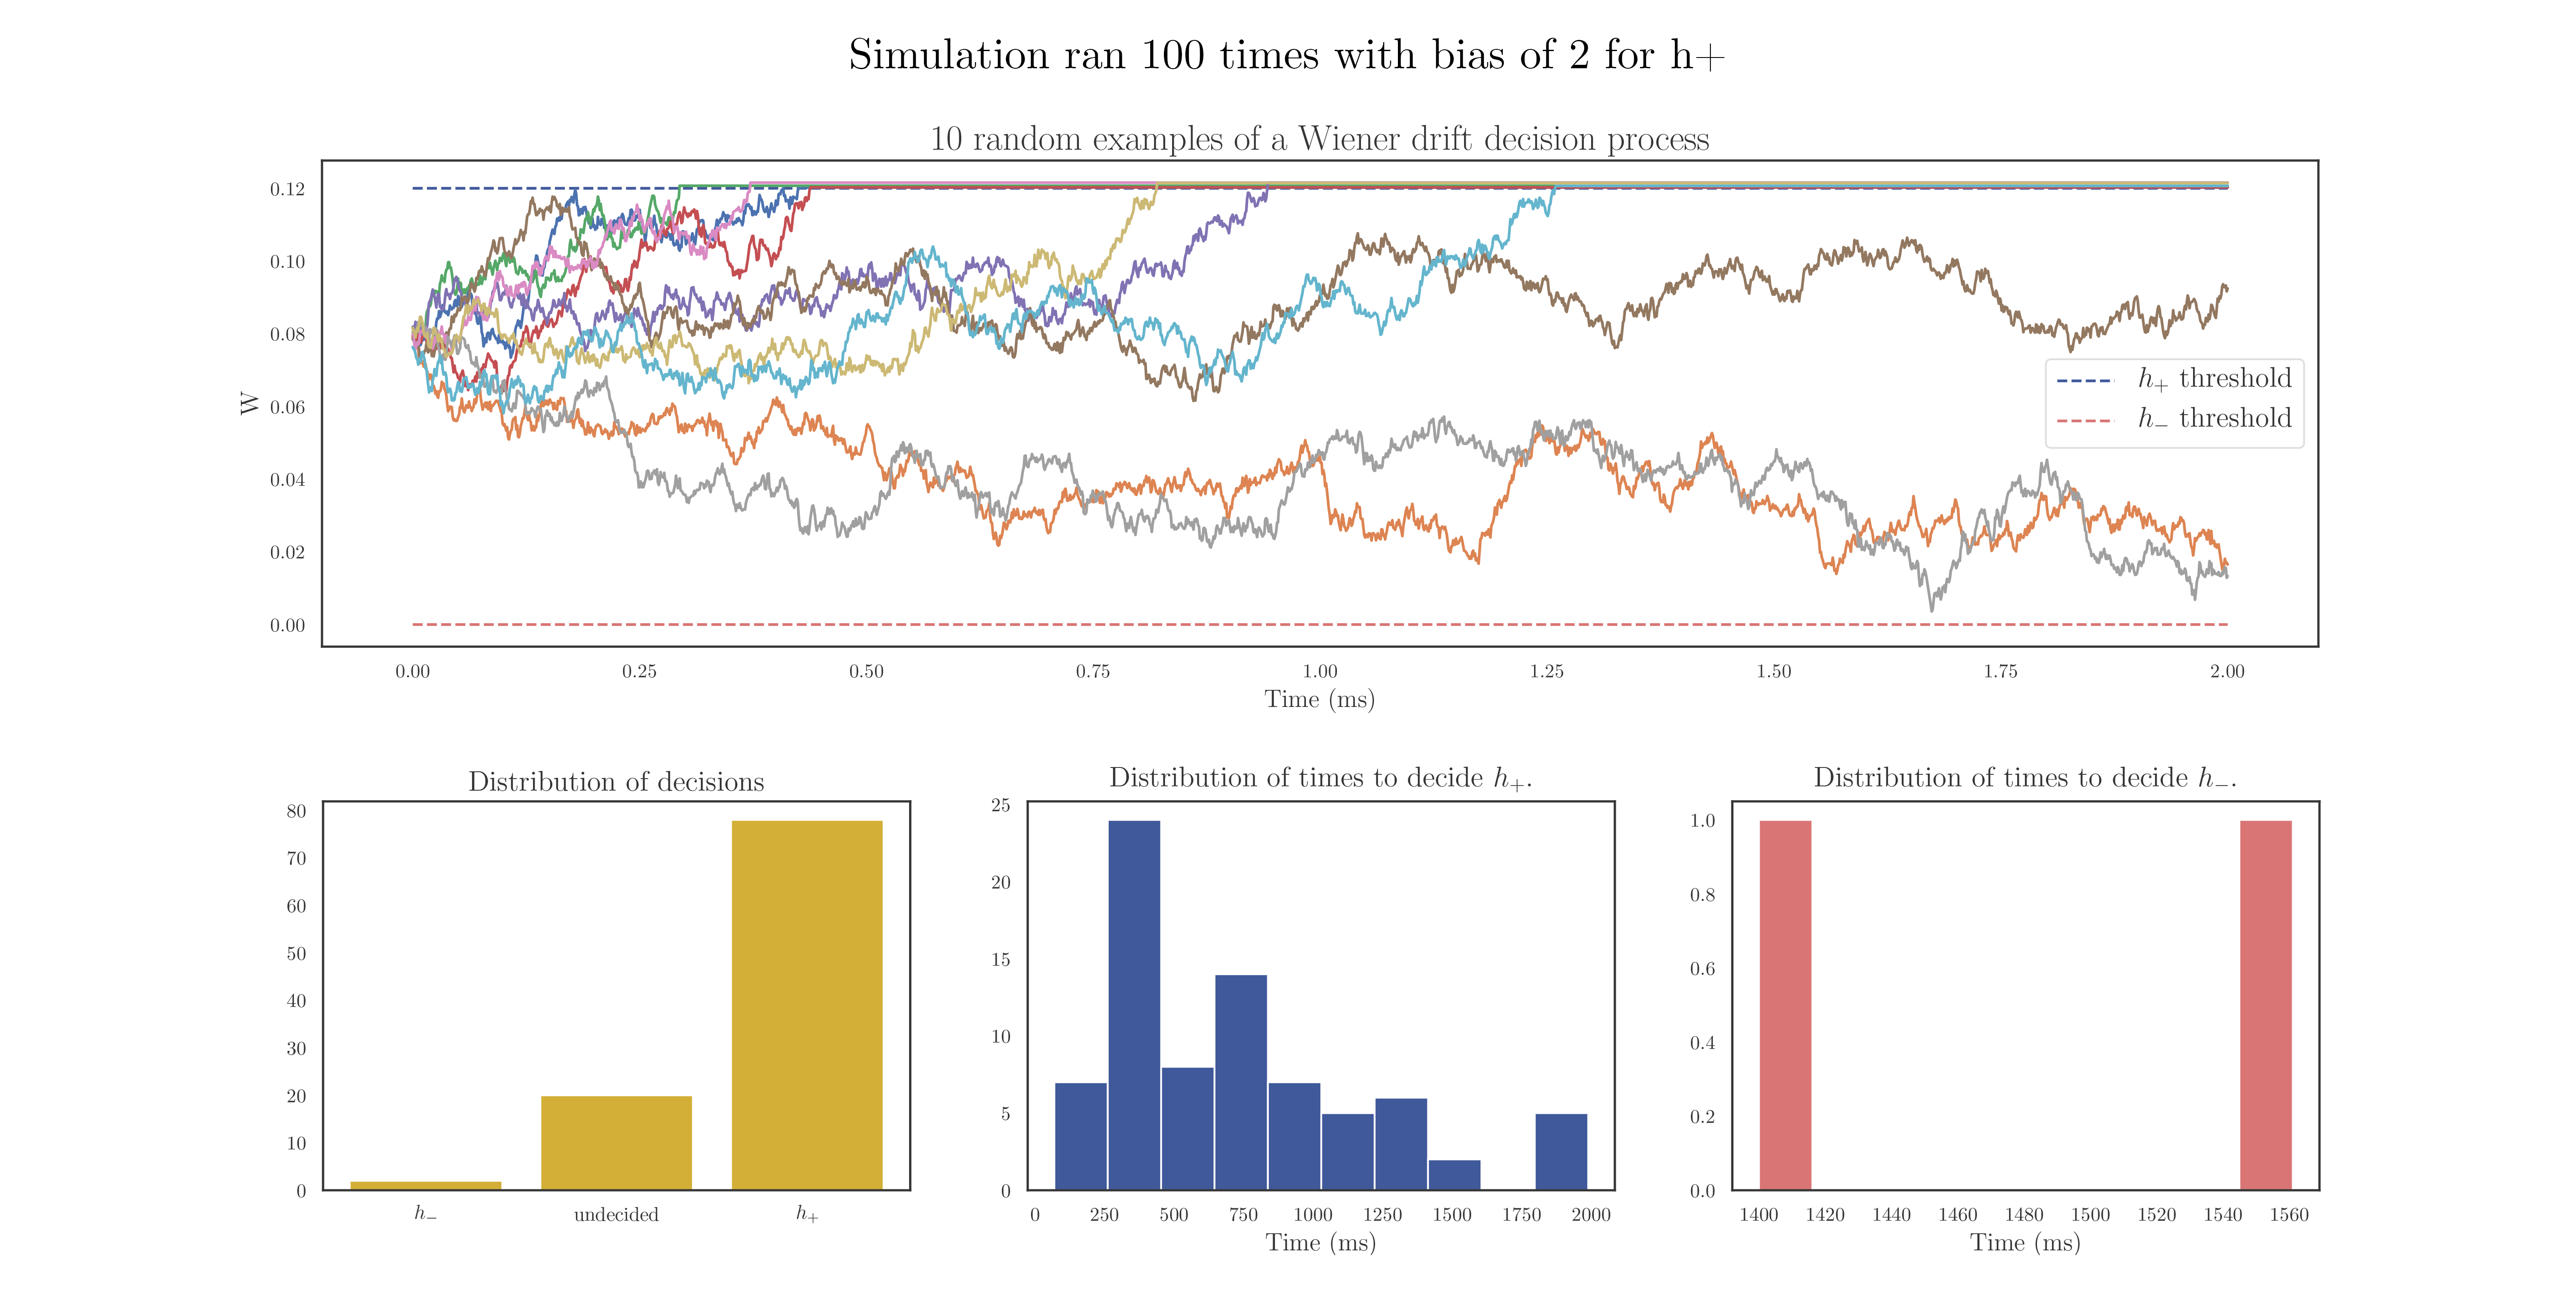
\includegraphics[width=1.2\linewidth]{figures/1-bias.png}
	\caption{Results of a drift-decision simulation ran 100 times with a drift-diffusion rate of 0.03, a boundary separation of 0.12 and a bias of 2 for $h^+$. Top: 10 randomly chosen decision paths. Bottom-left: Overall distribution of $h^+$, undecided and $h^-$. Bottom-centre: distribution of times to decide $h^+$. Bottom-right: distribution of times to decide $h^-$.}
	\label{fig:1-bias}
\end{figure}

Figure \ref{fig:1-bias} shows 10 random paths and the distributions of a simulation ran 100 times. In the paths we can see the new starting point. $h^+$ is selected 70\% of the times, compared to only 64\% without the bias. $h^-$ is chosen only 2\% of times. 

\section{Reinforcement learning models}

The behaviour of the participants was modelled using a reinforcement learning model, in which the value of the chosen stimulus $i$ was updates on trial $t$ after observing reward $r$ according to equation \ref{eq:0.0}. The initial values $V_0$ are set to 0.

\begin{equation}
    V_t^i = V_t^i + \epsilon + (r_t - V_t^i)
    \label{eq:0.0}
\end{equation}

The probability of choosing stimulus $A$ on trial $t$ is modelled by equation \ref{eq:0.1}

\begin{equation}
    P(\text{action } A | V_t, \beta) = \frac{\mathrm{exp}(\beta \times V_t^A)}{\mathrm{exp}(\beta \times V_t^A) + \mathrm{exp}(\beta \times V_t^B)}
    \label{eq:0.1}
\end{equation}


\subsection{Data exploration}

Before attempting to fit a model some data exploration was performed. Figure \ref{fig:2.1} shows the number of times each participant chose stimulus $A$, and the total number of rewards obtained. While participants who chose more times stimulus $A$ tend to have higher rewards, there is not a clear pattern observable in the figure. 

\begin{figure}[h!]
	\centering
	\hspace*{-0.6in}
	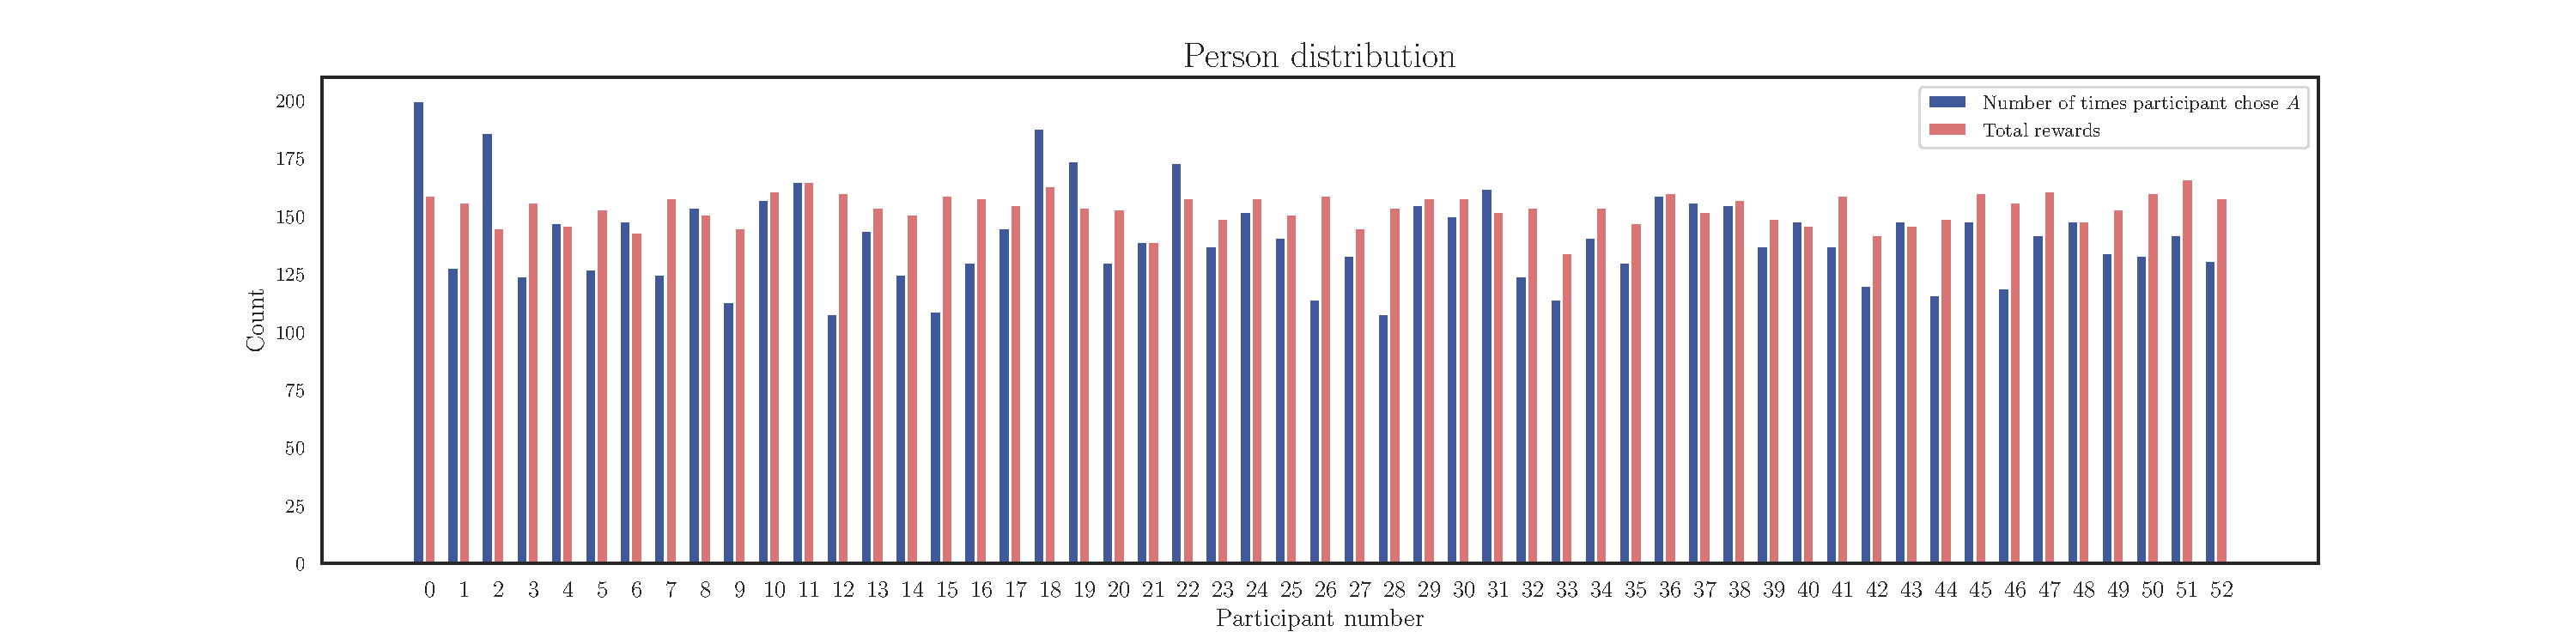
\includegraphics[width=1.2\linewidth]{figures/2.1.pdf}
	\caption{Plot of the total number of rewards and the number of times a participant chose stimulus $A$ for each participant.}
	\label{fig:2.1}
\end{figure}

The table below summarises the basic statistics for the studied variables. $A$ was chosen more than $50\%$ of the times, which is not surprising as, on average, choice $A$ had a higher probability of reward. The mean total rewards was 153.5, which is 64\% of the total.

The expected number of rewards if random choices were made can be obtained my

\[ \frac{\big(P(\mathrm{R} | A^1) + P(\mathrm{R} | B^1) + P(\mathrm{R} | A^2) + P(\mathrm{R} | B^2)\big) \times 100}{4} = 56.25 \]

Therefore, the expected number of rewards is lower than the average rewards obtained, which suggests that learning happened during the experiment.

\begin{center}
 \begin{tabular}{|c || c | c | c|} 
 \hline
  & Mean (out of 240) & Standard deviation & Range (out of 240) \\ [0.5ex] 
 \hline\hline
 Times $A$ was chosen & 141.0 & 20.31 & $[108, 200]$ \\ 
 \hline
 Total rewards & 153.5 & 6.63 & $[134,166]$ \\ [1ex] 
 \hline
\end{tabular}
\end{center}

\subsection{Simulated data exploration}

Figure \ref{fig:2.2} shows the average evolution of $V^A$, $V^B$ and $V^A - V^B$ for a simulation ran 100 times with 240 trials each. The trends clearly show that learning is happening with each probability switch, as when $V^A$ increases $V^B$ decreases and vice-versa. Moreover, it can be observer that when $P(\mathrm{R} | A) = 0.5 $ and $P(\mathrm{R} | B) = 0.75$ the learning happens slower than when $P(\mathrm{R} | A) = 0.75 $ and $P(\mathrm{R} | B) = 0.25$, as the difference in the probabilities is lower.

\begin{figure}[h!]
	\centering
	\hspace*{-0.4in}
	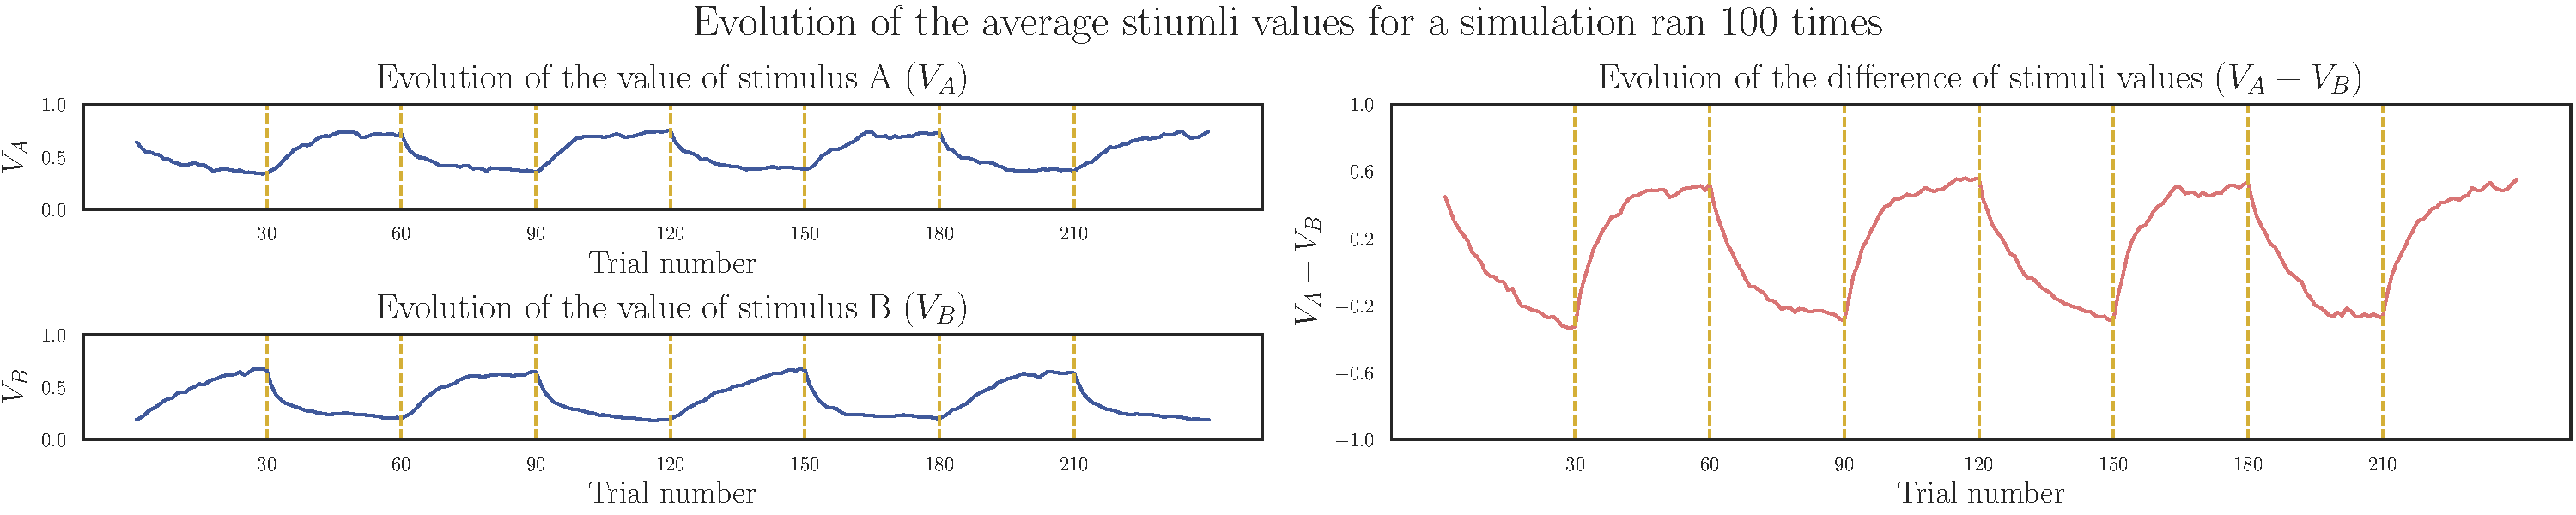
\includegraphics[width=1\linewidth]{figures/2.2.pdf}
	\caption{Plot of the average evolution of $V^A$ (top left), $V^B$ (bottom left) and $V^A - V^B$ (right), for a simulation ran 100 times with 240 trials. The golden dotted lines represent a switch in the probabilities.}
	\label{fig:2.2}
\end{figure}

The average number of rewards was 154.2.

\subsection{Parameter exploration}

For the parameter exploration, the values for the parameters were assigned:

\begin{description}
\item[$\epsilon_{\mathrm{values}}$:] linear space of 10 elements with range $[0, 1]$, 
\item[$\beta_{\mathrm{values}}$:] linear space of 15 elements with range $[1, 15]$.
\end{description}

Then, a simulation with 100 participants was performed for each pair of parameter values. 

\begin{figure}[h!]
	\centering
	\hspace*{-2.2in}
	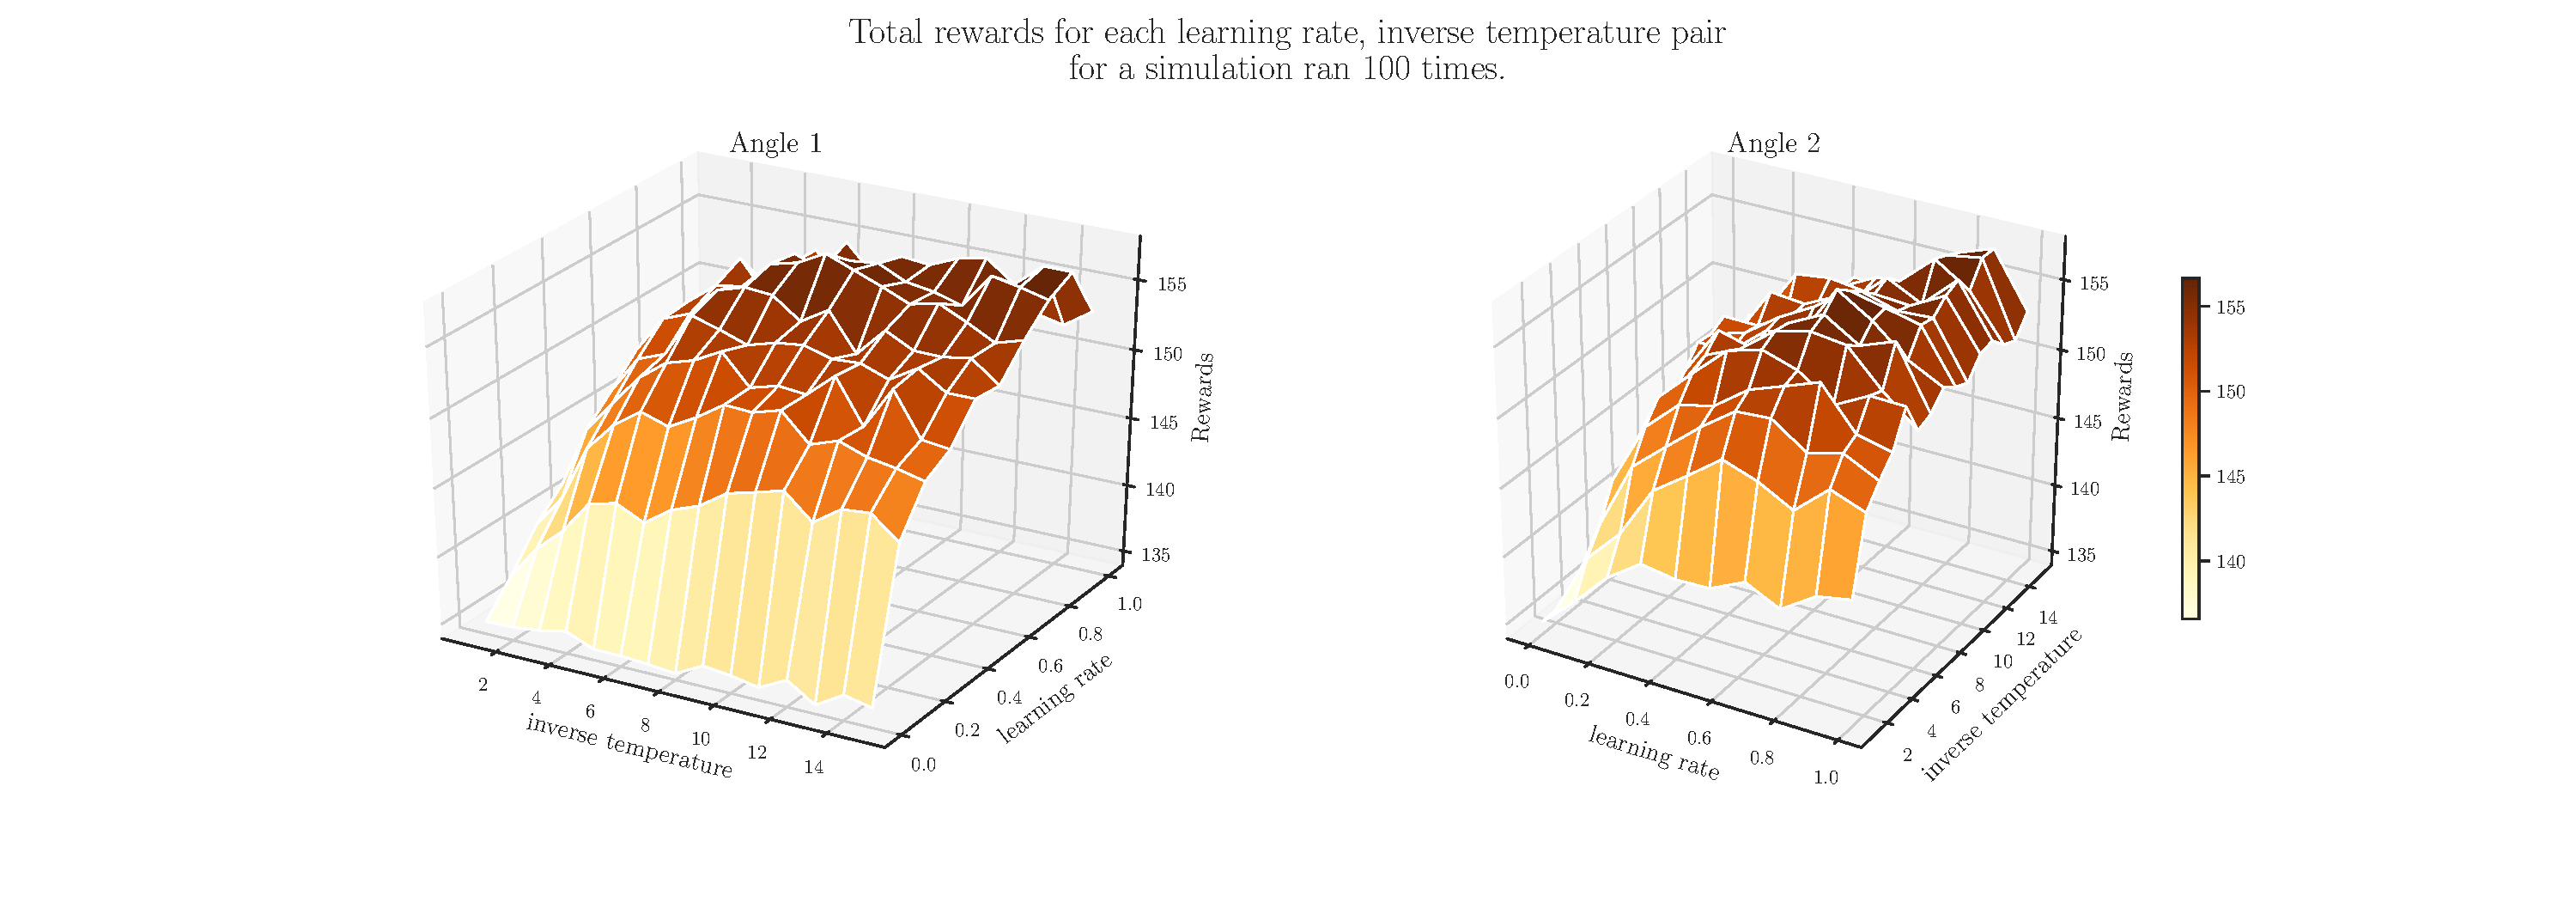
\includegraphics[width=1.5\linewidth]{figures/2.3.pdf}
	\caption{Plot of the number of rewards for each learning rate and inverse temperature pair. The two subplots correspond to two different angles to improve visibility.}
	\label{fig:2.3}
\end{figure}

Figure \ref{fig:2.3} shows the amount of reward of each pair of parameters. The reward increases as the inverse temperature increases from 0 to 10, and it stabilises afterwards. The learning rate also increases the reward as it increases up to a threshold of around 0.7, then the reward decreases as the learning rate increases.

\subsection{Negative log likelihood}

The negative log likelihood (NNL), using the formula provided in the report, was computed for the first participant, and it was 52 to two significant figures. 

For the second participant, the NNL was 63.83.

\subsection{Model fitting and group comparison}

\subsubsection{Model fitting}
\label{sec:fit-model-0}

The model was fit using the function \texttt{scipy.minimize} with the \texttt{BFGS} minimisation method \footnote{https://docs.scipy.org/doc/scipy/reference/generated/scipy.optimize.minimize.html}. $\epsilon = 0.5$ and $\beta = 5$ were used as starting parameters.

The minimisation algorithm encountered an overflow for most participants when running completely unconstrained. Therefore, the learning rate was constrained to being greater than 0, as there cannot be negative learning rates.

The mean learning rate (LR) found was 0.36, with a standard deviation of 0.123. The mean inverse temperature (IT) was 5.83, with a standard deviation of 1.25. 

\begin{figure}[h!]
	\centering
	\hspace*{-0.6in}
	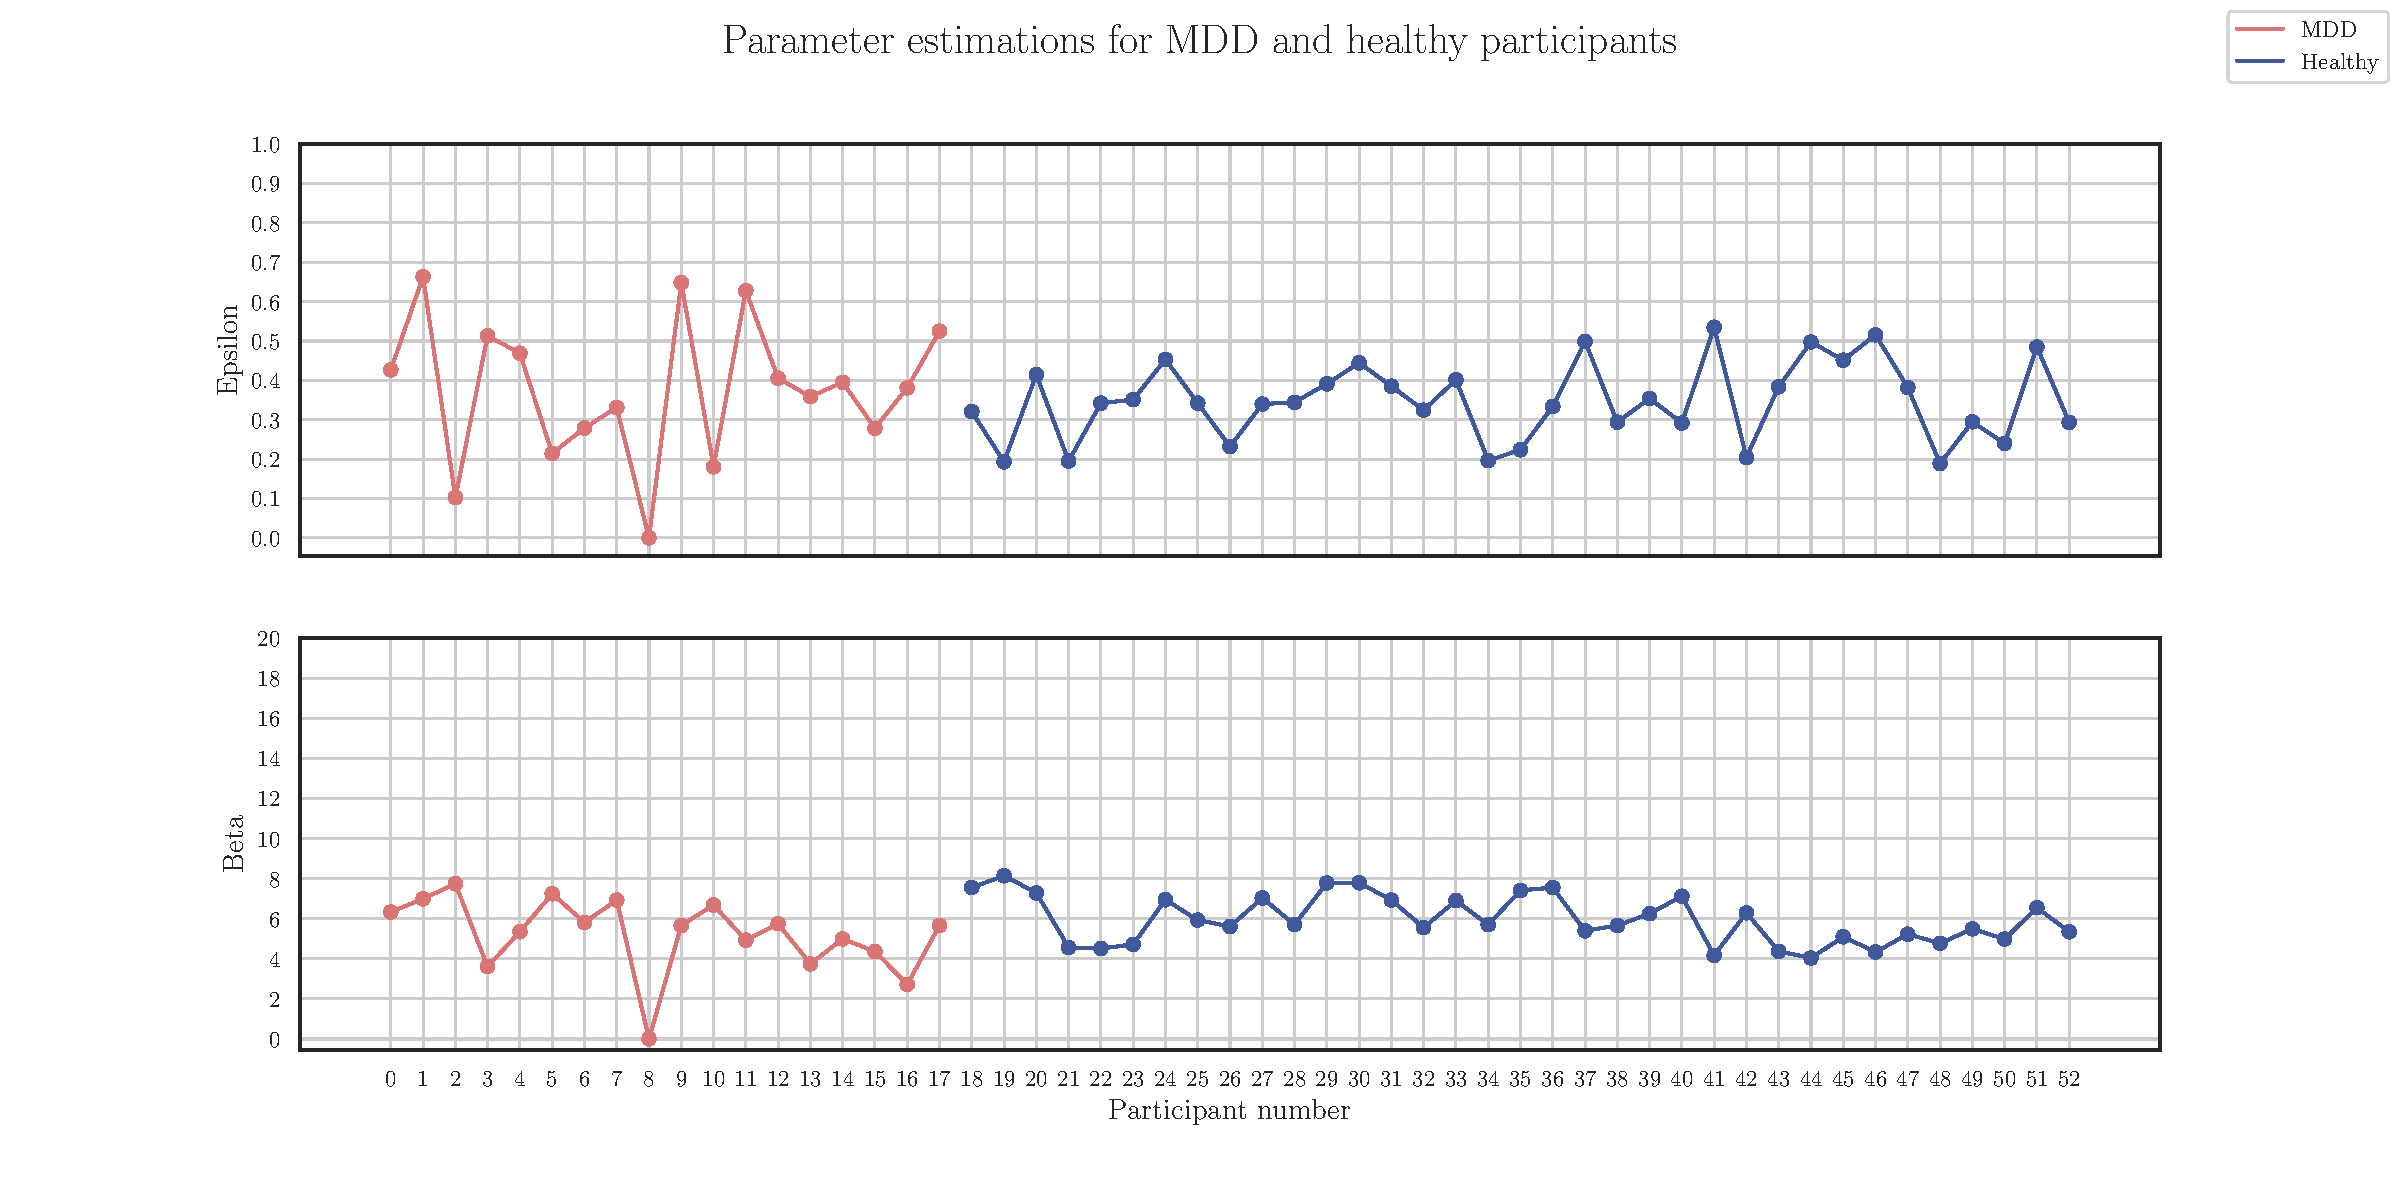
\includegraphics[width=1.1\linewidth]{figures/2.4.pdf}
	\caption{Best-fit learning rate (top) and inverse temperature (bottom) for healthy and MDD participants. The participants with 0 values were filtered-out because the best-fits were outside the normal range of $(0,1)$ for the LR and $(1, 15)$ for the IT.}
	\label{fig:2.4}
\end{figure}

Figure \ref{fig:2.4} shows the best-fit LR an IT for each participant, with considerably more variability in the MDD participants than in the healthy. It can also be observed that participant 8 has a value of 0 for both the LR and IT, this is because a filtering function was implemented to remove from the best-fit parameters those participants who did not fall within the normal range. The zero values seen in the plot are simply to keep the number of the participants constant, they were not taken into account for the reported statistics. 

Furthermore, the Pearson correlation coefficient was computed for all participants, and for the healthy and MDD participants together. The results can be seen in the table below. The p-value represents the probability that that the result would have been found if the correlation coefficient was 0.

\begin{center}
 \begin{tabular}{|c || c | c |} 
 \hline
  & Pearson correlation coefficient & p-value  \\ [0.5ex] 
 \hline\hline
 Overall & -0.22 & 0.11 \\ 
 \hline
 Healthy & -0.30 & 0.23 \\
 \hline
 MDD & -0.13 & 0.46 \\ [1ex] 
 \hline
\end{tabular}
\end{center}

There are no strong correlations between the best-fit LR and IT for any of the groups, which indicates that the optimisation algorithm functioned as expected, as high correlations would indicate anomalies in the data or the optimisation. 

\subsubsection{Group comparison}
\label{sec:t-model-0}
A two-sample T-test between the healthy and MDD groups was performed for both the LR and the EPS. The null hypothesis was that $\mu_{\mathrm{healthy}} = \mu_{\mathrm{MDD}}$. The degrees of freedom in both cases were 16 (as only 17 MDD patients were considered). The results of the T-statistic and the p-value can be seen in the table below:

\begin{center}
 \begin{tabular}{|c || c | c |} 
 \hline
  & T-statistic & p-value  \\ [0.5ex] 
 \hline\hline
 LR ($\epsilon$) & 1.33 & 0.19 \\
 \hline
 IT ($\beta$) & -0.66 & 0.51 \\ [1ex] 
 \hline
\end{tabular}
\end{center}

There is only a 0.19 probability that the null hypothesis is true for the LR, therefore we can probably reject the null hypothesis and say that there is a difference between both means.

On the other hand, for the IT there is a 0.51 probability that the null hypothesis is true. Thus, we cannot accept nor reject the null hypothesis or establish a difference between groups.

From the data, we would conclude that a reduced learning rate would be the differentiating factor between MDD and healthy participants.

Research about the effect of the LR has arrived to contradictory conclusions. \cite{chase2010approach} found a reduced learning rate in middle-aged MDD patients using a probabilistic selection task, which would be consistent with the findings in this report. However, \cite{gradin} found no difference in the LR between MDD patients and healthy controls, and \cite{dombrovski2010reward} found that there was only a difference between groups for the punishment LR, not the reward LR that is being considered in this report.

Moreover, \cite{series} found that the main impairments were the IT, which did not show as a differentiating factor in our findings, and a memory parameter that was not taken into account in our models.

\subsection{Parameter recovery}
\label{sec:recovery}

For the parameter recovery 53 pairs of parameters were obtained randomly from a normal distribution. Then, 53 sets of data each were simulated. For each set, the best-fit parameters were computed.

\begin{figure}[h!]
	\centering
	\hspace*{-0.6in}
	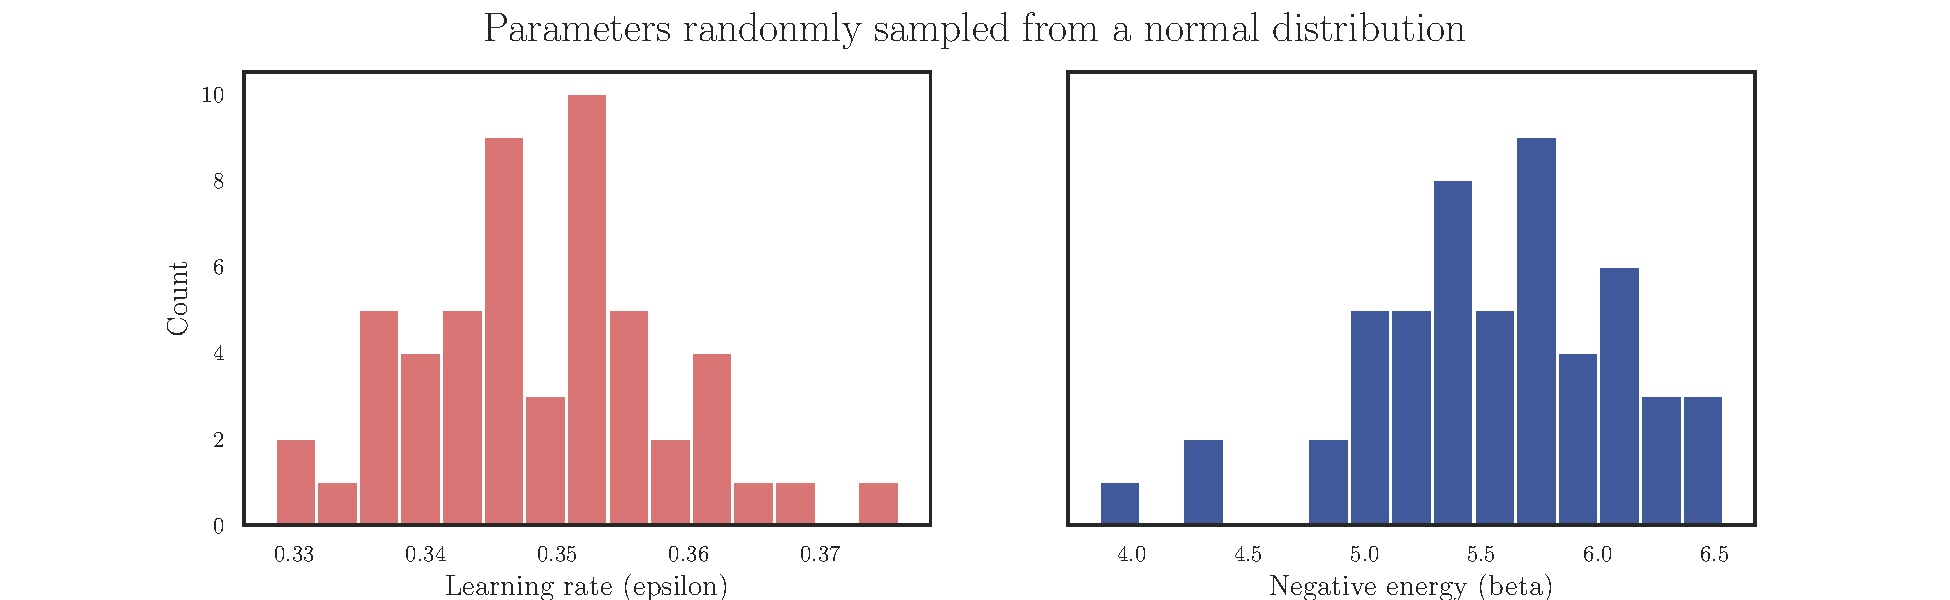
\includegraphics[width=1.15\linewidth]{figures/2.5.0.pdf}
	\caption{Distribution of the LR (left) and the IT (right) randomly sampled from normal distributions.}
	\label{fig:2.5.0}
\end{figure}


Figure \ref{fig:2.5.0} shows the distribution of the starting LRs and NEs. There are no values outside the expected ranges, thus no values were re-sampled.

The Pearson correlation coefficient between the starting and the best-fit LRs is 0.56, with a p-value of $10^{-16}$ there is a strong correlation with a very small probability that there is no correlation.

For the NEs, the Pearson correlation coefficient is 0.89 with a p-value of $10^{-19}$: the correlation is even stronger with a negligent probability that there is no correlation. The same information is illustrated in figure \ref{fig:2.5.1}

\begin{figure}[h!]
	\centering
	\hspace*{-0.6in}
	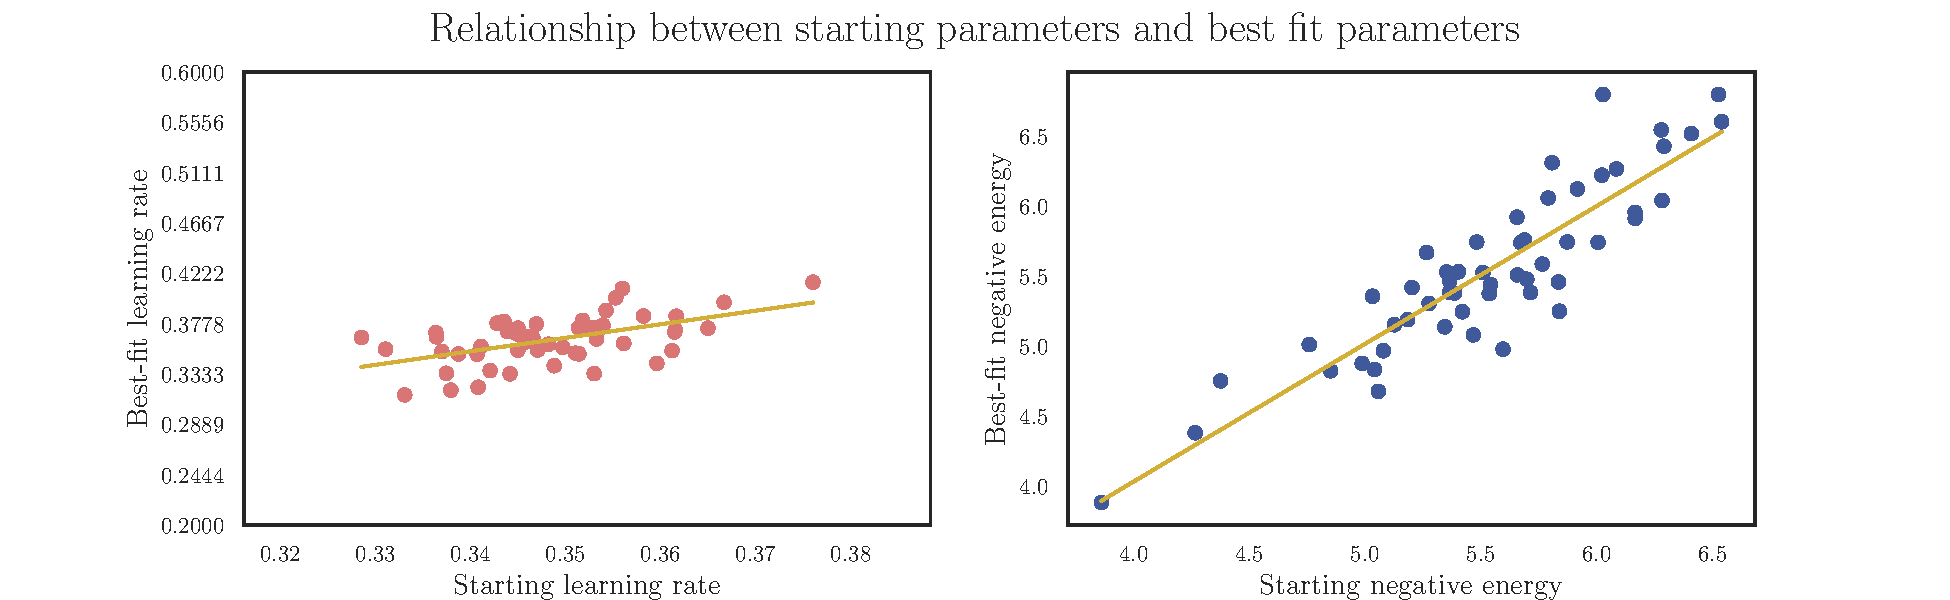
\includegraphics[width=1.15\linewidth]{figures/2.5.1.pdf}
	\caption{Relationship between the randomly sampled starting parameters and the best-fit parameters between for the LR (left) and the IT (right). The golden line represents the line of best fit.}
	\label{fig:2.5.1}
\end{figure}

\subsection{Additional models}

Two additional models were considered to fit the data. The first model got rid of the inverse temperature parameter (equation \ref{eq:1.1} when calculating the probability and introduced a new parameter when calculating the reinforcement learning values: a reward sensitivity (RS) parameter (equation \ref{eq:1.0}). The second model used the same equations as the initial one, but it has initial reinforcement learning values other $V_0 = (V^A_0, V^B_0)$. 

\begin{equation}
    V_t^i = V_t^i + \epsilon + (\rho \times r_t - V_t^i)
    \label{eq:1.0}
\end{equation}

\begin{equation}
    P(\text{action } A | V_t) = \frac{\mathrm{exp}(V_t^A)}{\mathrm{exp}(V_t^A) + \mathrm{exp}(V_t^B)}
    \label{eq:1.1}
\end{equation}

\subsubsection{Model 1}

To fit the model 1 the starting parameters chosen were $\epsilon=0.5$, as in model 0, and $\rho=5.5$, as given in the course lectures.

The table below shows the Pearson correlation coefficient between the two fit parameters for all participants, healthy participants, and MDD participants. There is not a strong correlation between any, which, as discussed in section \ref{sec:fit-model-0}, was expected.

\begin{center}
 \begin{tabular}{|c || c | c | c| c |} 
 \hline
  & Pearson correlation coefficient & p-value  \\ [0.5ex] 
 \hline\hline
 Overall & -0.21 & 0.14  \\ 
 \hline
 Healthy & -0.13 & 0.48 \\
 \hline
 MDD & -0.33 & 0.48 \\ [1ex] 
 \hline
\end{tabular}
\end{center}

\begin{figure}[h!]
	\centering
	\hspace*{-0.6in}
	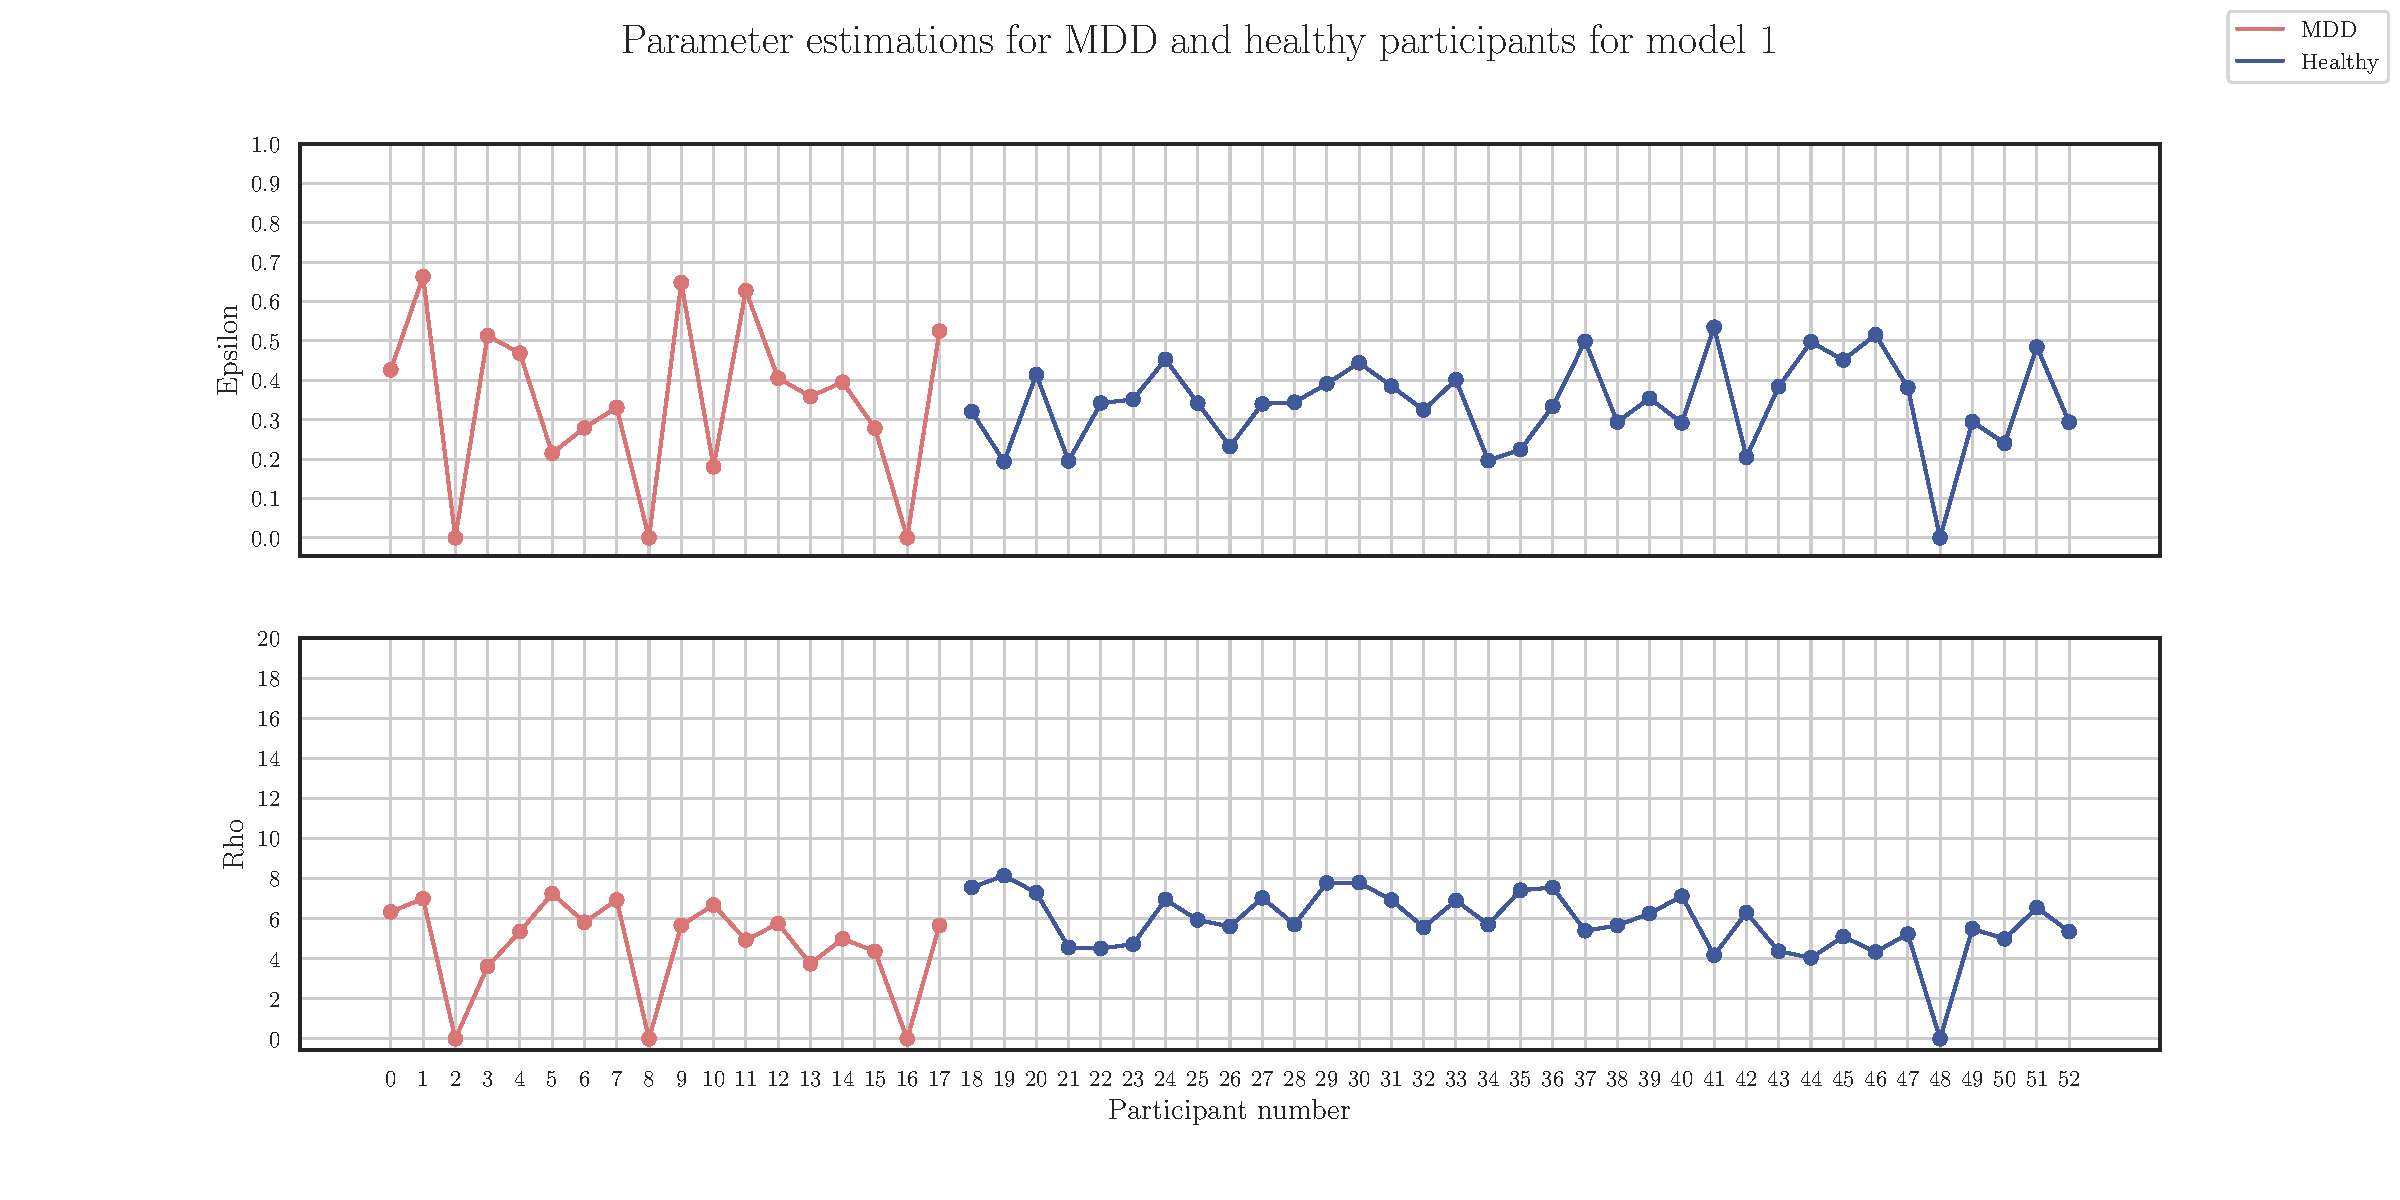
\includegraphics[width=1.1\linewidth]{figures/2.6.1.pdf}
	\caption{Best-fit learning rate (top) and inverse temperature (bottom) for healthy and MDD participants. The participants with 0 values were filtered-out because the best-fits were outside the normal range of $(0,1)$ for the LR and $(1, 15)$ for the IT.}
	\label{fig:2.6.1}
\end{figure}

Figure \ref{fig:2.6.1} shows the best fit LR and RS for all participants. It can be observed that more participants had values outiside the normal range and had to be discarded than with model 0. There is a lot more variability between MDD than between healthy participants for the LR, which was to be expected from model 0. The distribution of the RS, however, seems to be very similar between groups. A two sample T-test as in section \ref{sec:t-model-0} was performed to get better insights about the group differences. The results can be seen in the table below.

\begin{center}
 \begin{tabular}{|c || c | c |} 
 \hline
  & T-statistic & p-value  \\ [0.5ex] 
 \hline\hline
 LR ($\epsilon$) & 1.33 & 0.19 \\
 \hline
 RS ($\rho$) & 0.31 & 0.76 \\ [1ex] 
 \hline
\end{tabular}
\end{center}


There is a statistically significant difference between the menans of the LR for healthy and MDD participants at an 80\% confidence level. However, there seems to be no difference in the RS between the groups. These results were surprising as research has found that when performing a probabilistic reward task to asses reward learning, participants with MDD had reduced reward sensitivity and hence performed worse \cite{rho} .

\subsubsection{Model 2}

To fit the model 2 the $\epsilon$ and $\beta$ parameters were 0.5 and 5.5 respectively, as in model 0. However, the starting reinforcement learning values were $(0.3, 0.1)$. $A$ was given a bigger starting value than $B$ because the there is a bias in the given probabilities towards choice $A$. 

The table below shows the Pearson correlation coefficient between the two fit parameters for all participants, healthy participants, and MDD participants. As with the previous two models, there are no strong correlations.

\begin{center}
 \begin{tabular}{|c || c | c | c| c |} 
 \hline
  & Pearson correlation coefficient & p-value  \\ [0.5ex] 
 \hline\hline
 Overall & -0.26 & 0.07  \\ 
 \hline
 Healthy & -0.13 & 0.46 \\
 \hline
 MDD & -0.34 & 0.16 \\ [1ex] 
 \hline
\end{tabular}
\end{center}

\begin{figure}[h!]
	\centering
	\hspace*{-0.6in}
	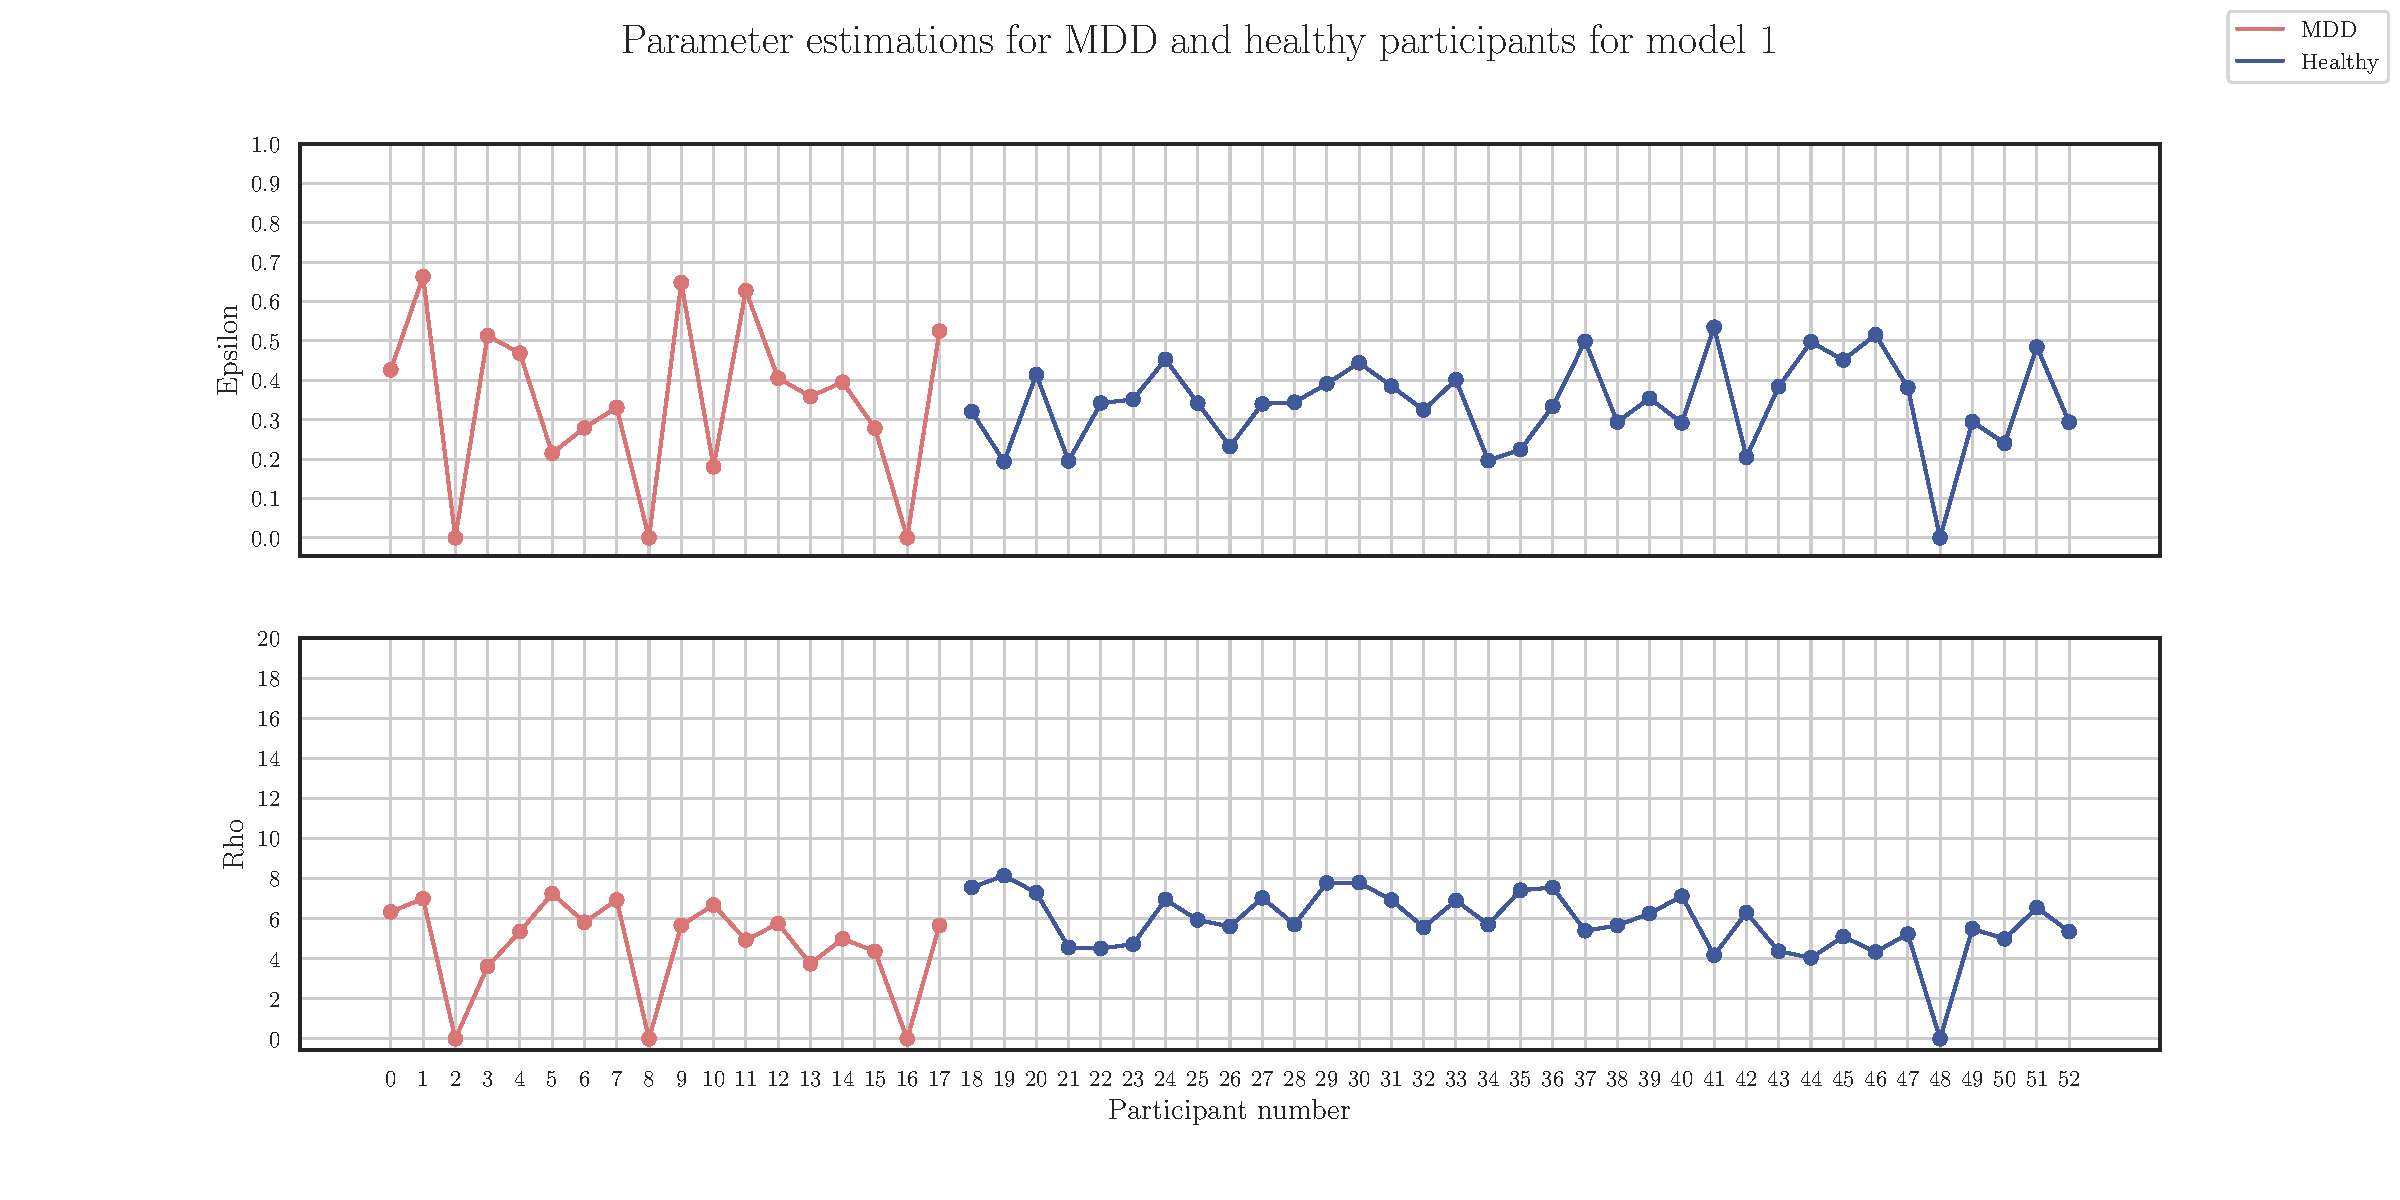
\includegraphics[width=1.1\linewidth]{figures/2.6.1.pdf}
	\caption{Best-fit learning rate (top) and inverse temperature (bottom) for healthy and MDD participants. The participants with 0 values were filtered-out because the best-fits were outside the normal range of $(0,1)$ for the LR and $(1, 15)$ for the IT.}
	\label{fig:2.6.2}
\end{figure}

Figure \ref{fig:2.6.2} shows the best-fit parameters for all participants. We can, again, observe more variability between groups in the LR than in the IT, which seems to be uniform. The results of the two-sample T-test can be seen below.

\begin{center}
 \begin{tabular}{|c || c | c |} 
 \hline
  & T-statistic & p-value  \\ [0.5ex] 
 \hline\hline
 LR ($\epsilon$) & 1.51 & 0.14 \\
 \hline
 IT ($\beta$) & -0.5 & 0.61 \\ [1ex] 
 \hline
\end{tabular}
\end{center}

As in the previous two models, there is a statistically significant difference between groups at an 86\% confidence level for the LR. There does not seem to be a difference for the IT.

\subsection{Model Comparison}
\label{sec:model-comparison}
To perform model comparison the data was fit using the three models. Then, for each model the $AIC$ and $BIC$ scores were computed to see which model fit the data best. 

Each of the three models was fit, the negative log likelihood was computed, and the scores for each model were obtained using equations \ref{eq:aic} and \ref{eq:bic}.

\begin{equation}
\label{eq:aic}
AIC = \sum_{\forall \mathrm{ppts}} 2 \times NLL + 2 p = 2 p \times |\mathrm{ppts}|  + 2 \sum_\mathrm{\forall \mathrm{ppts}} NLL
\end{equation}

\begin{equation}
BIC = \sum_{\forall \mathrm{ppts}} 2 \times NLL + 2 \log(n) =  p \times \log(n) \times |\mathrm{ppts}|  + 2 \sum_\mathrm{\forall \mathrm{ppts}} NLL
\label{eq:bic}
\end{equation}

The results are shown in the table below.


\begin{center}
 \begin{tabular}{|c || c | c | c |} 
 \hline
  & Model 0 & Model 1 & Model 2  \\ [0.5ex] 
 \hline\hline
 $AIC$ & 8377 & 8633 & 8610 \\
 \hline
 $BIC$ & 33129 & 33385 & 33362 \\ [1ex] 
 \hline
\end{tabular}
\end{center}

According to the material in lectures, there is a winning model if the difference in scores between models is $\>$ 10. However, since we have added scores for 53 participants, we would expect a difference between models $\> 530$. Model 0 has the lowest scores, but greatest difference between any Model 0 scores and any other score is always smaller than 300. Therefore, we can conclude that Model 0 might be the best-fitting model, further exploration would be necessary.

\subsection{Model recovery}

To perform model recovery, for each model 50 sets of data with 53 participants each were generated, using parameters extracted from a normal distribution as in section \ref{sec:recovery}. Then, for each data-set, the three models were fit to find the best-fitting parameters. Thus, for each model we had 50 data sets, and for each data set three sets of best fitting parameters.

Then, a confusion matrix was generated to report, for each model that generated the data, which of the three models fit the data better. The comparison was done using the same methods as in section \ref{sec:model-comparison}. The results of the confusion matrix can be seen in the table below:

\vspace{0.3in}

\begin{center}
\setlength\unitlength{1cm}
\begin{picture}(4,4)
\multiput(0.1,0.1)(0,1){4}{\line(1,0){3}}
\multiput(0.1,0.1)(1,0){4}{\line(0,1){3}}
\put(0.25,0.5){0.42}
\put(1.25,0.5){0.06}
\put(2.25,0.5){0.52}

\put(0.25,1.5){0.06}
\put(1.25,1.5){0.90}
\put(2.25,1.5){0.04}

\put(0.25,2.5){0.50}
\put(1.25,2.5){0.08}
\put(2.25,2.5){0.42}

\put(-0.5,2.5){0}
\put(-0.5,1.5){1}
\put(-0.5,0.5){2}

\put(0.5,3.5){0}
\put(1.5,3.5){1}
\put(2.5,3.5){2}

\put (-1.2,0){\rotatebox{90}{Generator model}}
\put(0.3,4.2){Best-fit model}
\end{picture}
\end{center}

The confusion matrix shows that, while when model 1 generates the data it is the best fitting model 90\% of the time, there is a big overlap between models 0 and 2. 

When model 0 generates the data, only 50\% of the time it is the best-fit model, while model 2 is 42\% of the time. Similarly, when Model 2 generates the data it is the best-fit model 52\% of the time, while Model 1 is 42\%. This shows that there is not a big distinction between models 0 and 2. 

Therefore, given these results, models 0 and 2 could be assumed to be the same. This would leave us with only models 0 and 1, which would make the results in the last section (discarding those for model 2) reliable.

Further research should concentrate in trying other starting parameters for model 2 to see if there could be a difference, or improvement, with model 0. 

\subsection{Discussion}

In this section, we defined a reinforcement learning model with two parameters, LR and IT, to understand the learning impairments in MDD participants when completing a probabilistic decision task. 

First, the model was fit and parameter recovery was performed to see that the model was suitable for the amount of data available. We then introduced two additional models, which were fit to the data without performing parameter recovery. Finally, the model recovery was done to obtain the best-fitting model. 

Instead, it might have been more insightful to perform parameter recovery for all models first, to assess whether they were suitable. Then, perform model recovery to have a simulated model comparison. This could have given insights about which model would be the best before performing the analysis with the real data. 

Concerns were raised about the realism of performing this 240-trial tasks without breaks with severely-ill participants. 

One potential solution would be reducing the trials by half. To assess the solution, parameter recovery was performed as in section \ref{sec:recovery}, but with 120 trials per participant instead of 240. The Pearson correlation coefficient was 0.20 and 0.57 for the learning rate and the inverse temperature respectively. There is correlation between the starting and best-fit LRs; which shows that with that solution we would be missing data.

Another solution proposed was to give the participants a break halfway through. The task is designed such that the participants learn as the task goes by. The success in each trial depends strongly on the events that have happened right before the trial. Therefore, pausing in the middle of the task would disrupt the flow, potentially making the participants forget about the previous states and depriving them from learning.

If participants had to respond within a brief time window there would have to be changes in the simulation and the model. First, assuming that participants, on average, skipped 5\% of trials due to the time limit, when generating simulated data we would have to delete trials with a 5\% probability. Then, we would probably have to modify our models and add a new parameter that represents the effect of pressure, as there is a chance that the pressure affects MDD and healthy participants different.

If the experiment also included punishments, new parameters would have to be introduced. Model 1 would also need a punishment sensitivity parameter. The hypotheses for all models would change, as some research has found that the LR for punishment is impaired in MDD patients, but not the LR for reward (see \cite{dombrovski2010reward}). Therefore, new hypothesis that differentiate the effect of the learning rate when punishing or rewarding would also be needed.


\bibliography{bib}

\end{document}
